\section{Evaluation}\label{sec:eval}

To evalute feature-sensitive coverages, we apply $\tool$ to the latest language
specification (ES13, 2022)~\cite{es13} with different $k$-FS and $k$-FCPS
node-or-branch coverages to synthesize JavaScript conformance tests.
%
As a result, we synthesize \inred{185,246} conformance tests using $\tool$ with
five different graph coverage criteria: 1) a node-or-branch coverage and 2)
1-FS, 3) 2-FS, 4) 1-FCPS, and 5) 2-FCPS node-or-branch coverages.
%
Our evaluation platform is a 4.0GHz Intel(R) Core(TM) i7-6700k and 32GB of RAM
(Samsung DDR4 2133MHz 8GB*4), and it takes \inred{72} hours to synthesize
conformance tests.
%
We evaluated the synthesized conformance test suite with the following four
research questions:
\begin{itemize}
  \item \textbf{RQ1 (Conformance Bug Detection):} How many conformance bugs of
    JavaScript engines and transpilers do conformance tests synthesized by
    $\tool$ detect? (Section~\ref{sec:conform-bug})
  \item \textbf{RQ2 (Impact of $k$-FS Coverages):} What effect do $k$-FS
    coverages have in detecting conformance bugs?
    (Section~\ref{sec:impact-k-fs})
  \item \textbf{RQ3 (Impact of $k$-FCPS Coverages):} What effect do $k$-FCPS
    coverages have in detecting conformance bugs compared to $k$-FS coverages?
    (Section~\ref{sec:impact-k-fcps})
  \item \textbf{RQ4 (Comparison with Test262):} Could conformance tests
    synthesized by $\tool$ improve Test262, the official JavaScript conformance
    suite maintained by hand? (Section~\ref{sec:compare-test262})
\end{itemize}

%----------------------------------------%
%----------------------------------------%

\subsection{Conformance Bug Detection}\label{sec:conform-bug}

\begin{table}
\caption{
  Detected conformance bugs in JavaScript engines and transpilers.
}
\vspace*{-.5em}
{
\small
\label{tab:conform-bugs}
\begin{tabular}{?c?l|l|l?r|r|r?}
\toprule\\[-1.6em]

\multicolumn{1}{?c?}{\multirow{2}{*}{\textbf{Kind}}}
& \multicolumn{1}{c|}{\multirow{2}{*}{\textbf{Name}}}
& \multicolumn{1}{c|}{\multirow{2}{*}{\textbf{Version}}}
& \multicolumn{1}{c?}{\multirow{2}{*}{\textbf{Release}}}
& \multicolumn{3}{c?}{\textbf{\# Detected Unique Bugs}} \\\cline{5-7}

&&&
& \multicolumn{1}{c|}{\textbf{\# New}}
& \multicolumn{1}{c|}{\textbf{\# Confirmed}}
& \multicolumn{1}{c?}{\textbf{\# Reported}}\\

\toprule\\[-1.6em]

\multirow{5}{*}{Engine}
& V8            & v10.8.121 & 2022.10.06 & \x{0} & \x{0} & \x{3} \\\cline{2-7}
& JSC           & v615.1.10 & 2022.10.26 & \x{4} & \x{4} & \x{14}\\\cline{2-7}
& GraalJS       & v22.2.0   & 2022.07.26 & \x{7} & \x{7} & \x{9} \\\cline{2-7}
& SpiderMonkey  & v107.0b4  & 2022.10.24 & \x{1} & \x{3} & \x{3} \\\cline{2-7}
& \multicolumn{3}{c?}{\textbf{Total}}    & \y{12}& \y{14}& \y{29}\\

\toprule\\[-1.6em]

\multirow{5}{*}{Transpiler}
& Babel         & v7.19.1   & 2022.09.15 & \x{33}& \x{33}& \x{39}\\\cline{2-7}
& SWC           & v1.3.10   & 2022.10.21 & \x{30}& \x{30}& \x{32}\\\cline{2-7}
& Terser        & v5.15.1   & 2022.10.05 & \x{1} & \x{1} & \x{15}\\\cline{2-7}
& Obfuscator    & v4.0.0    & 2022.02.15 & \x{0} & \x{0} & \x{3} \\\cline{2-7}
& \multicolumn{3}{c?}{\textbf{Total}}    & \y{64}& \y{64}& \y{89}\\

\toprule\multicolumn{1}{c}{}\\[-1.6em]


\multicolumn{4}{?c?}{\textbf{Total}}
& \y{76}& \y{78}& \y{118}\\

\toprule\multicolumn{1}{c}{}\\[-1.6em]
\end{tabular}
}
\end{table}

%----------------------------------------%

Using the synthesized JavaScript conformance tests, we check the conformance of
eight mainstream tools (four engines and four transpilers) listed in
Table~\ref{tab:conform-bugs}.
%
We select them as evaluation targets because they support all the language
features in ES13.
%
V8, JSC, and SpiderMonkey are JavaScript engines used in web browsers, Google
Chrome, Apple Safari, and Mozilla Firefox, respectively.
%
GraalJS is a JavaScript engine built on GraalVM, a JDK distribution developed by
Oracle written for JVM languages along with support for cloud-native and
polyglot.
%
Babel and SWC are transpilers that desugar new language features into old ones,
usually ES5.1 features, for legacy host environments.
%
Terser is a code compressor that reduces the code size by removing code
fragments, making names smaller, or inlining variable references.
%
Finally, JavaScript Obfuscator obfuscates code to make it hard to understand and
reverse-engineering.

%----------------------------------------%

Table~\ref{tab:conform-bugs} gives the distribution of the detected conformance
bugs by \inred{185,246} synthesized conformance tests.
%
We found conformance bugs in all the evaluation targets using the synthesized
conformance tests.
%
In addition, we manually inspected the failed conformance test cases,
categorized them as \inred{118} unique conformance bugs, and reported them to
the developers of the target tools.
%
As a result, \inred{78} out of \inred{118} bugs were officially confirmed, and
\inred{76} were newly discovered bugs.
%
The other \inred{40} reported bugs are still under review, or developers have
not yet responded.
%
Among \inred{118} detected bugs, \inred{29} are engine bugs, and \inred{118} are
transpiler bugs.
%
The two most trusted engines are V8 and SpiderMonkey because they have only
three conformance bugs.
%
Hence, we use V8 as the default engine during the transpiler conformance check.
%
If V8 fails a conformance test, we use another JavaScript engine that passes the
test for the conformance check of a transpiler.
%
Among transpilers, Terser and JavaScript Obfuscator contain only \inred{15} and
\inred{3} bugs, respectively, but Babel and SWC have \inred{39} and
\inred{32} transpiler conformance bugs, respectively.
%
It happens because transpilers desugaring new language features to ES5.1
features is more challenging than compressing or obfuscating the code.

%----------------------------------------%
%----------------------------------------%

\subsection{Impact of $k$-FS Coverages}\label{sec:impact-k-fs}

\begin{table}
\caption{
  Comparison of synthesized conformance test suite guided by five different
  graph coverage criteria: 1) a node-or-branch coverage, and 2) 1-FS, 3) 2-FS,
  4) 1-FCPS, and 5) 2-FCPS node-or-branch coverages.
}
\vspace*{-.5em}
{
\small
\label{tab:compare}
\begin{tabular}{?c?r|r|r?r|r?}
\toprule\\[-1.6em]

\multicolumn{1}{?c?}{\multirow{2}{*}{\textbf{coverage criterion}}}
& \multicolumn{3}{c?}{\textbf{\# covered TRs (K)}}
& \multicolumn{1}{c|}{\multirow{2}{*}{\textbf{\# syn. tests}}}
& \multicolumn{1}{c?}{\multirow{2}{*}{\textbf{\# bugs}}}\\\cline{2-4}

& \multicolumn{1}{c|}{\textbf{\# nodes}}
& \multicolumn{1}{c|}{\textbf{\# branchs}}
& \multicolumn{1}{c?}{\textbf{\# total}}
&&\\

\toprule\\[-1.6em]

node-or-branch
& \x{2.1}     & \x{10.0}    & \x{12.1}    & \x{2,095} & \x{45}  \\\hline
1-FS node-or-branch
& \x{61.5}    & \x{34.2}    & \x{95.7}    & \x{5,336} & \x{60}  \\\hline
2-FS node-or-branch
& \x{1,131.5} & \x{663.3}   & \x{1,794.8} & \x{83,668}& \x{115} \\\hline
1-FCPS node-or-branch
& \x{257.7}   & \x{133.2}   & \x{390.9}   & \x{5,446} & \x{75}  \\\hline
2-FCPS node-or-branch
& \x{2,854.9} & \x{1,500.4} & \x{4,355.3} & \x{88,701}& \x{118} \\

\toprule\multicolumn{1}{c}{}\\[-1.6em]

\end{tabular}
}
\end{table}

%----------------------------------------%

To evaluate the effect of $k$-FS coverages, we compare the synthesized
conformance tests guided by different $k$-FS normal-or-branch coverage criteria.
%
Table~\ref{tab:compare} shows the result of conformance test synthesis via
$\tool$ with five different graph coverage criteria: 1) a node-or-branch
coverage and 2) 1-FS, 3) 2-FS, 4) 1-FCPS, and 5) 2-FCPS node-or-branch
coverages.
%
The first three columns denotes the number of covered $k$-FS or $k$-FCPS nodes
(\textbf{\# nodes}), branches (\textbf{\# branches}), and any TRs (\textbf{\#
total}).
%
The fourth and fifth columns denote the number of synthesized conformance tests
(\textbf{\# syn. tests}) and the number of detected unique bugs by synthesized
tests (\textbf{\# bugs}).

%----------------------------------------%

According to the table's first to third rows, the number of covered
TRs increased \inred{7.91x (95.7K / 12.1K)} from baseline to 1-FS coverage and
\inred{18.8x (1794.8K / 95.7K)} from 1-FS to 2-FS coverages.
%
The difference between 1-FS and 2-FS coverages is much higher than between
baseline and 1-FS.
%
It is due to that many abstract algorithms in the language specification are
related to the limited number of language features, while most language features
could enclose diverse language features.
%
For a more detailed information, we draw histograms of numbers of 1-FS-TRs per
baseline TR and 2-FS-TRs per 1-FS-TR in Figures~\ref{fig:hist} (a) and (b).
%
The most significant number of 1-FS-TRs per baseline TR is \inred{X for a node
in the X abstract algorithm because all the X utilize the X algorithm to define
their semantics in the language specification.}
%
The most significant number of 2-FS-TRs per 1-FS-TR is \inred{X for a node whose
most enclosing feature is X because diverse X use X.}
%
The number of synthesized tests increased \inred{2.55x (5,336 / 2,095)} from
0-FS to 1-FS coverages and \inred{15.7x (83,668 / 5,336)} from 1-FS to 2-FS
coverages.
%
In addition, the number of detected unique bugs also increased when using higher
$k$-FS normal-or-branch coverages.
%
The baseline with a simple node-or-branch coverage detects \inred{45}
conformance bugs in engines and transpilers.
%
The conformance tests synthesized with 1-FS coverage detect \inred{15 (60 - 45)}
more conformance bugs, and tests synthesized with 2-FS coverage detect \inred{55
(115 - 60)} more bugs.

%----------------------------------------%

\textbf{Empty Name Binding for \jscode{let} in \jscode{for}-Loops.}
%
ES13 provides diverse shapes of $\jscode{for}$-loops as syntactic features
defined with the \esnt{ForStatement} syntactic production.
%
Among them, a \jscode{for}-loop with a \jscode{let}-binding is a syntactic
feature for its third alternative.
%
While it normally has one or more name bindings, we could pass an empty list of
name bindings using an empty object destructuring pattern: \jscode{\{\}}.
%
However, Babel v7.19.1 crashes when transpiling a \jscode{for}-loop with
empty name bindings for \jscode{let}, such as a JavaScript program in
Listing~\ref{lst:empty-let-bug}.
%
While the semantics that checks the empty name bindings is described in the
\textbf{CreatePerIterationEnvironment} algorithm, other language features also
utilize it when defining their semantics.
%
Hence, we failed to detect this conformance bug using the tests synthesized with
a simple node-or-branch coverage.
%
On the other hand, feature-sensitive coverages could discriminate the usage of
empty name binding checking semantics in different language features.
%
As a result, we successfully detected this conformance bug with 1-FS, 2-FS,
1-FCPS, or 2-FCPS coverages.
\begin{lstlisting}[style=JS,numbers=left,frame=single,
caption={A crashing bug in Babel v7.19.1.},
label={lst:empty-let-bug}
]
// [EXIT] Normal
for (let {} = 0; 0; ) ;
\end{lstlisting}

%----------------------------------------%

\todo\ for 2-FS

%----------------------------------------%
%----------------------------------------%

\subsection{Impact of $k$-FCPS Coverages}\label{sec:impact-k-fcps}

\begin{figure}
  \centering
  \begin{subfigure}{0.24\textwidth}
    \centering
    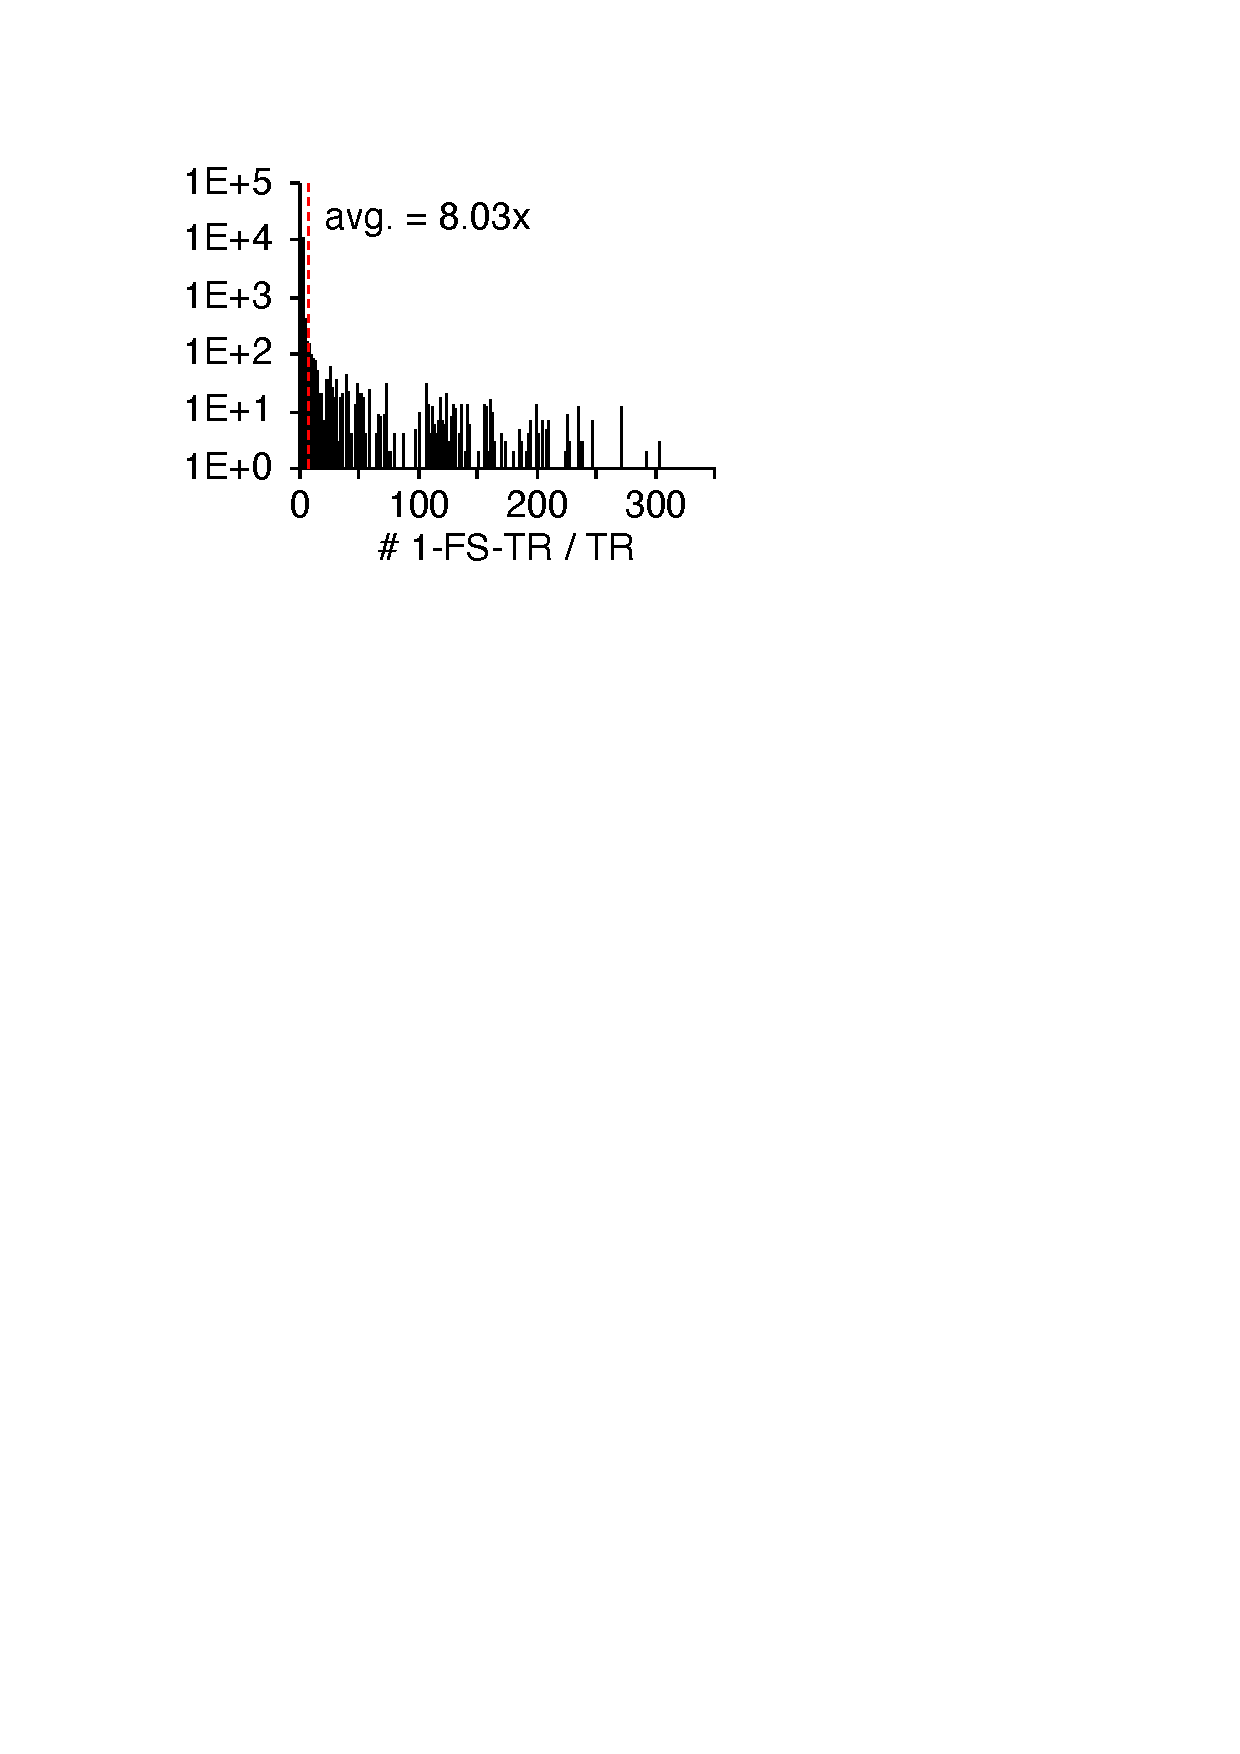
\includegraphics[width=\textwidth]{img/1-fs-hist}
    \subcaption{\#1-FS-TRs / base TR.}
  \end{subfigure}
  \begin{subfigure}{0.24\textwidth}
    \centering
    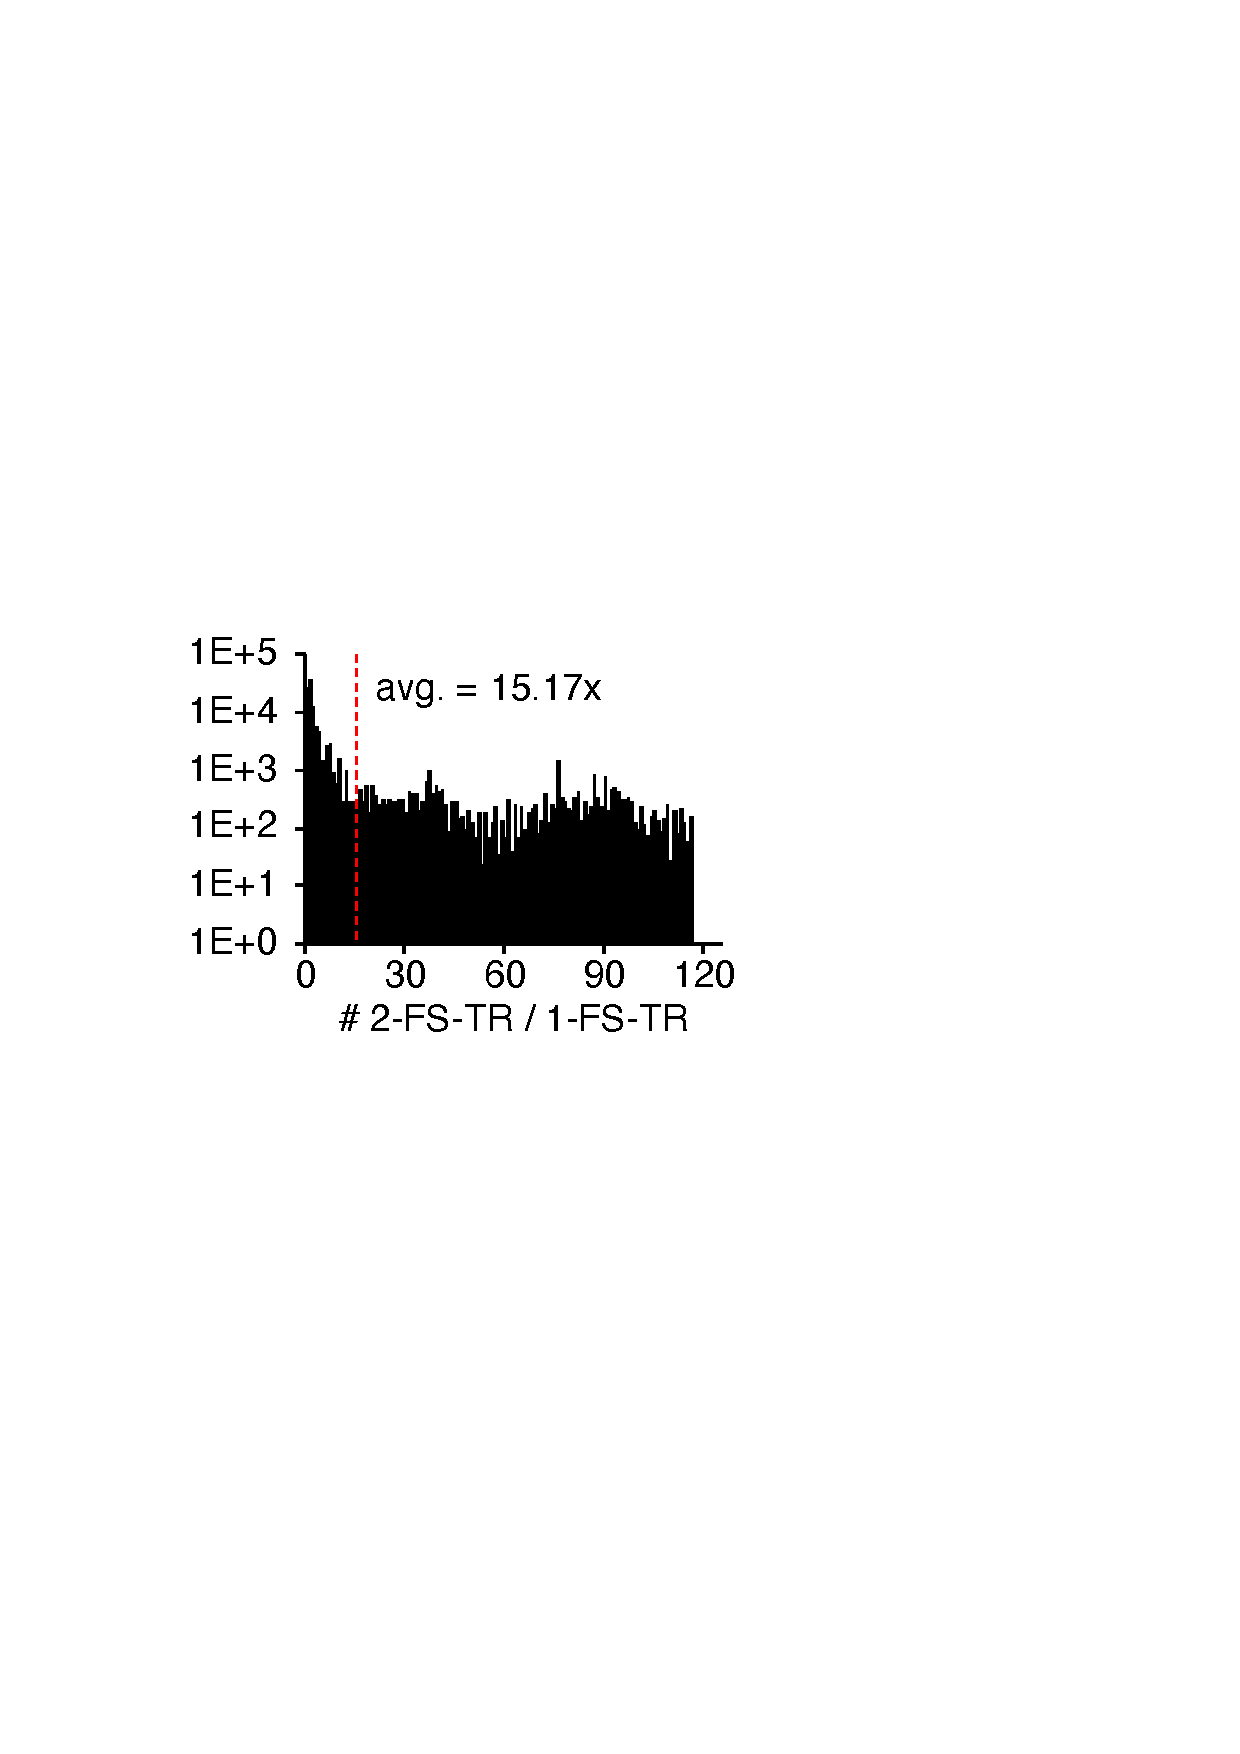
\includegraphics[width=\textwidth]{img/2-fs-hist}
    \subcaption{\#2-FS-TRs / 1-FS-TR.}
  \end{subfigure}
  \begin{subfigure}{0.24\textwidth}
    \centering
    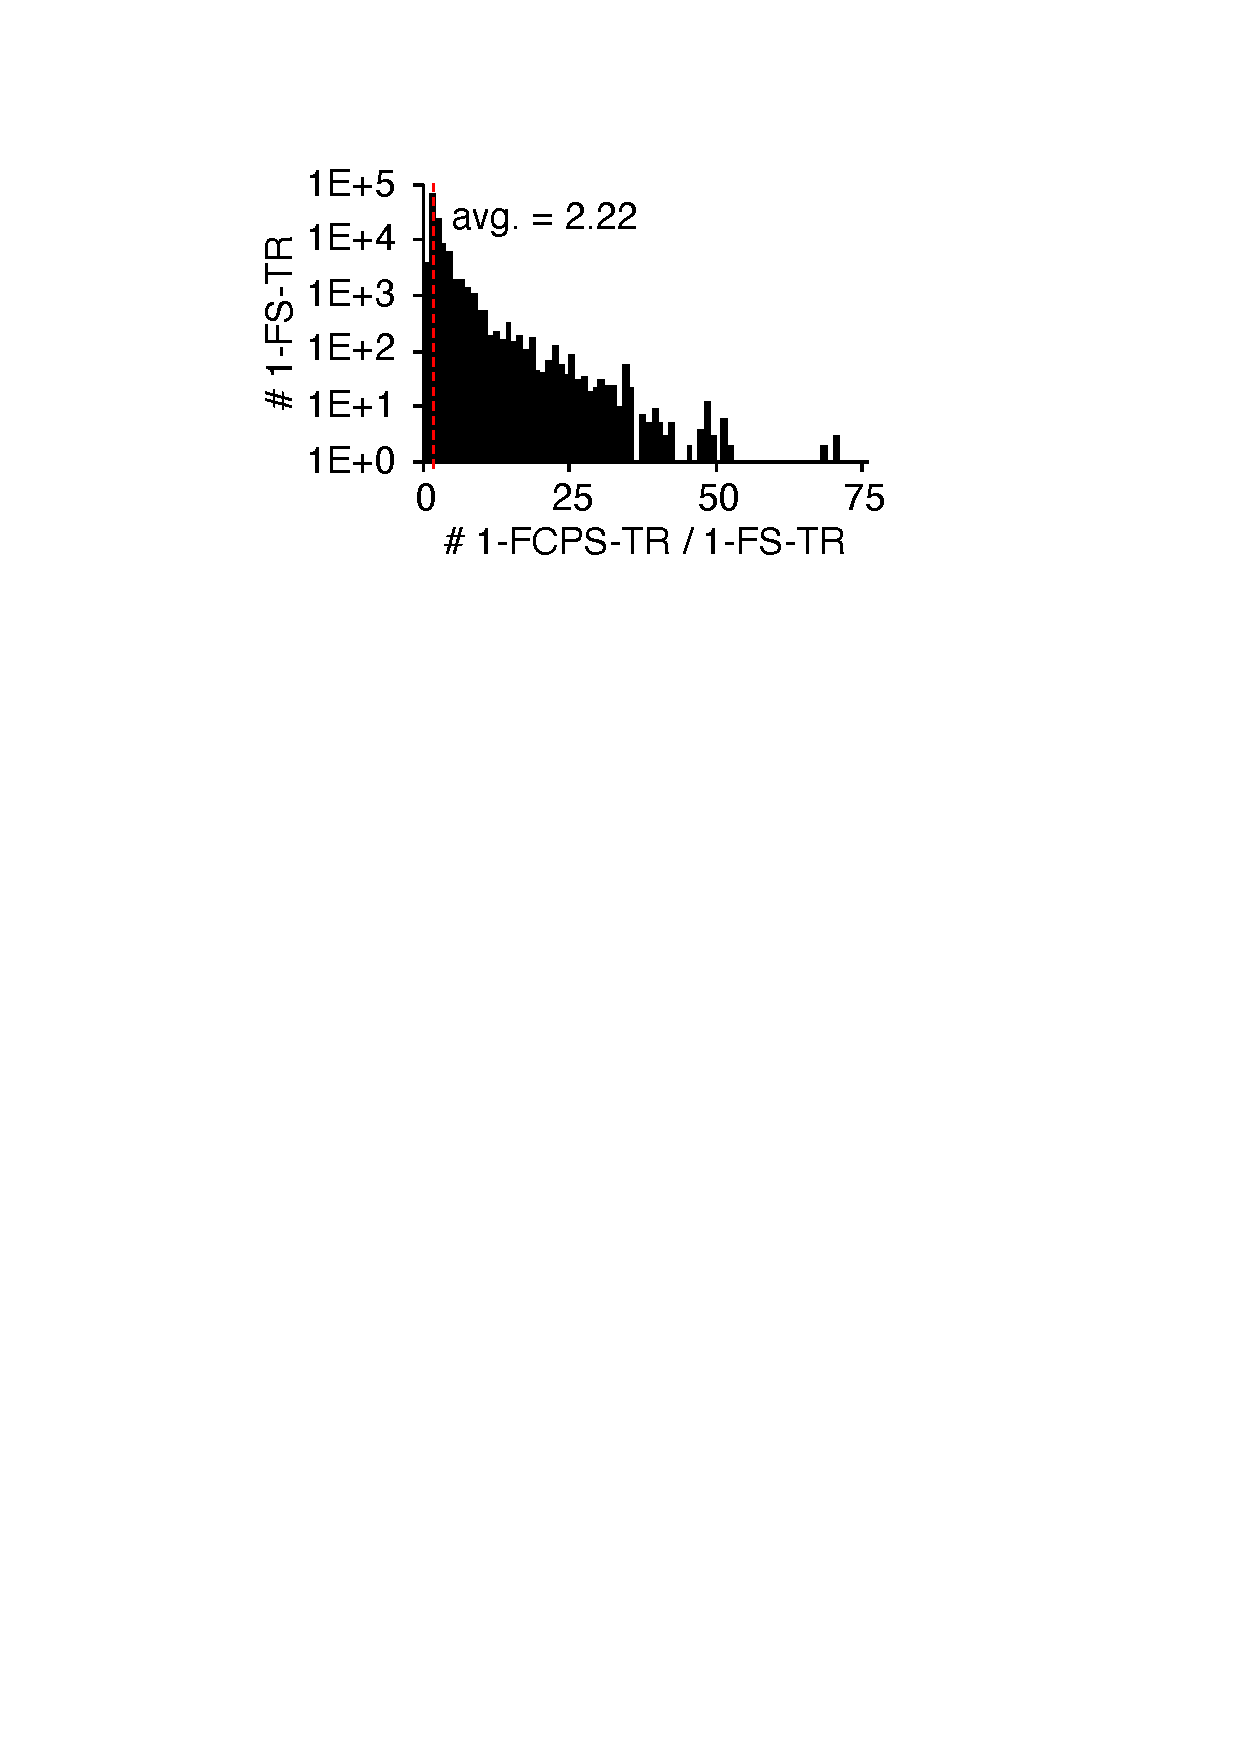
\includegraphics[width=\textwidth]{img/1-fcps-hist}
    \subcaption{\#1-FCPS-TRs / 1-FS-TR.}
  \end{subfigure}
  \begin{subfigure}{0.24\textwidth}
    \centering
    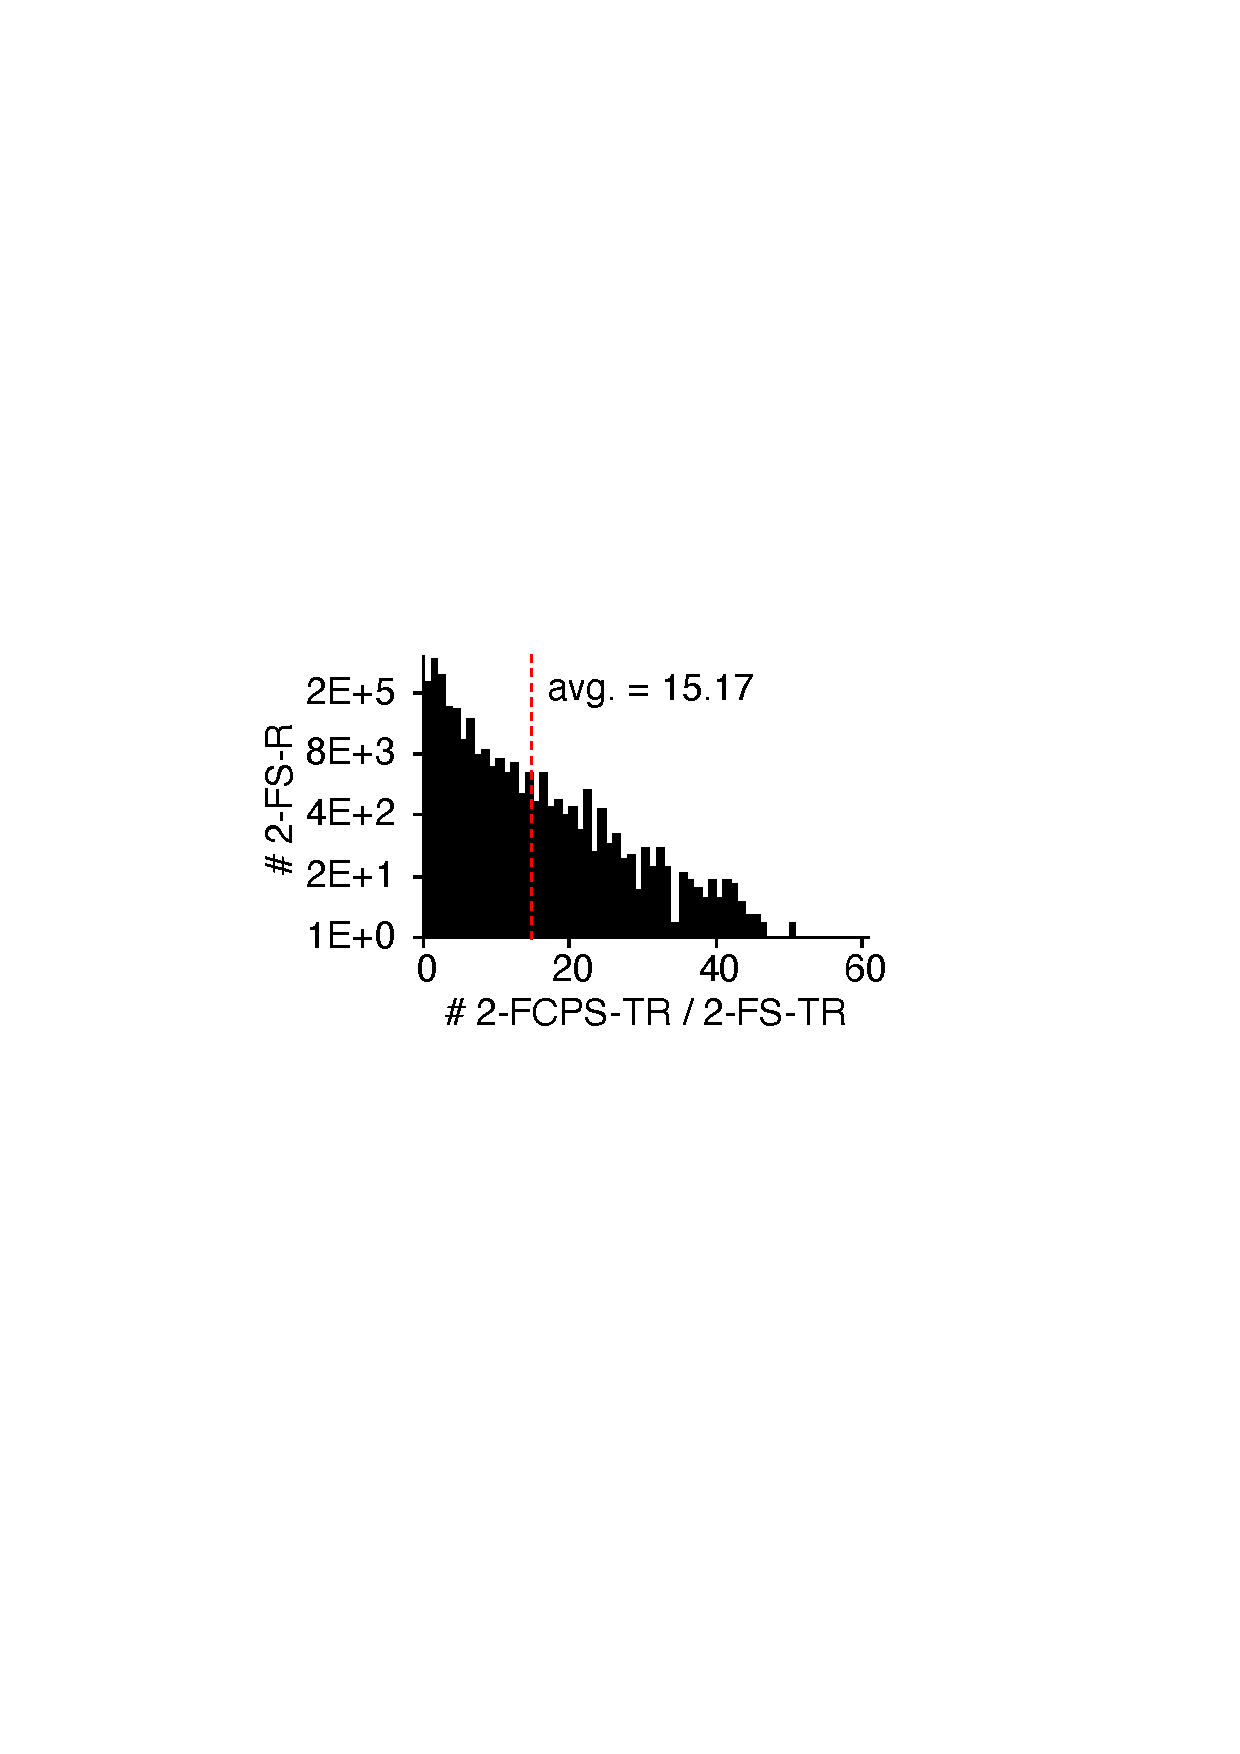
\includegraphics[width=\textwidth]{img/2-fcps-hist}
    \subcaption{\#2-FCPS-TRs / 2-FS-TR.}
  \end{subfigure}
  \caption{
    The histogram of numbers of $k$-FS or $k$-FCPS TRs per less sensitive $k$-FS
    or $k$-FCPS TR.
  }
  \label{fig:hist}
\end{figure}

%----------------------------------------%

We also evaluate the effect of $k$-FCPS coverages compared to $k$-FS coverages.
%
According to the second to fifth rows in Table~\ref{tab:compare}, $\tool$ covers
\inred{4.08x (390.9K / 95.7K)} and \inred{2.43x (4355.3/1794.8)} more TRs when
using $k$-FCPS coverages instead of $k$-FS coverages for $k = 0$ and $k = 1$,
respectively.
%
Figures~\ref{fig:hist} (c) and (d) provide more detailed information about the
increment of covered TRs.
%
Each of them depicts the histogram of numbers of 1-FCPS-TRs (or 2-FCPS-TRs) per
1-FS-TR (or 2-FS-TR).
%
The most significant number of 1-FCPS-TRs per 1-FS-TR is \inred{X for a node in
the X abstract algorithm whose most enclosing feature is X.}
%
\inred{In the semantics of the X feature, the X abstract algorithm used in X,
which increases the number of feature call paths.}
%
The most significant number of 2-FCPS-TRs per 2-FS-TR is \inred{X for a node
whose most enclosing feature is X for the same reason.}
%
Because of the increased number of TRs, the number of synthesized tests also
increased \inred{2.55x (5,336 / 2,095)} from 0-FS to 1-FS coverages and
\inred{15.7x (83,668 / 5,336)} from 1-FS to 2-FS coverages.
%
In addition, the number of detected unique bugs also increased when using
$k$-FCPS coverages than $k$-FS coverages for the same $k$.
%
The conformance tests synthesized with 1-FCPS and 2-FCPS coverages detect
\inred{15 (75 - 60)} and \inred{3 (118 - 115)} more conformance bugs than 
1-FS and 2-FS coverages, respectively.
%
Now, we introduce two bug examples to show the effect of $k$-FCPS coverages
compared to the $k$-FS coverages.

%----------------------------------------%

\todo\ for 1-FCPS

% XXX appeared not only in 1-FCPS and 2-FCPS but also in 1-FS and 2-FS
% \paragraph{\textbf{\jscode{String.prototype.normalize}}}
% The \jscode{String.prototype.normalize} built-in API normalizes a given string
% into the normalization form named by a given argument.
% %
% For example, \jscode{"abc".normalize("NFC")} produces the NFC normalization form
% of "abc".
% %
% If an invalid name as the argument, it should throws a \textbf{RangeError}.
% %
% However, the JavaScript program in Listing~\ref{lst:normalize-bug} noramlly
% terminates in GraalJS v22.2.0 while it should throw a \textbf{RangeError}
% because of the invalid name \jscode{""}.
% %
% While it covers a specific branch in \textbf{ToString} abstract algorithm, the
% semantics of \jscode{String.prototype.normalize} built-in API also utilizes this
% algorithm to get a string from the \jscode{this} value.
% %
% Therefore, we failed to detect this conformance bug by the tests synthesized
% with baseline or $k$-FS coverages.
% %
% On the other hand, feature call paths could discriminate two different
% invocations of the \textbf{ToString} algorithm, and we successfully detected
% this conformance bug with 1-FCPS and 2-FCPS coverages.
% 
% \begin{lstlisting}[style=JS,numbers=left,frame=single,
% caption={Expected a \textbf{RangeError} but normally terminated in GraalJS
% v22.2.0.},
% label={lst:normalize-bug}
% ]
% // [EXIT] RangeError
% String.prototype.normalize.call(0, "");
% \end{lstlisting}

%----------------------------------------%

\todo\ for 2-FCPS

%----------------------------------------%
%----------------------------------------%

\subsection{Comparison with Test262}\label{sec:compare-test262}

\begin{figure}
  \centering
  \begin{subfigure}{0.19\textwidth}
    \centering
    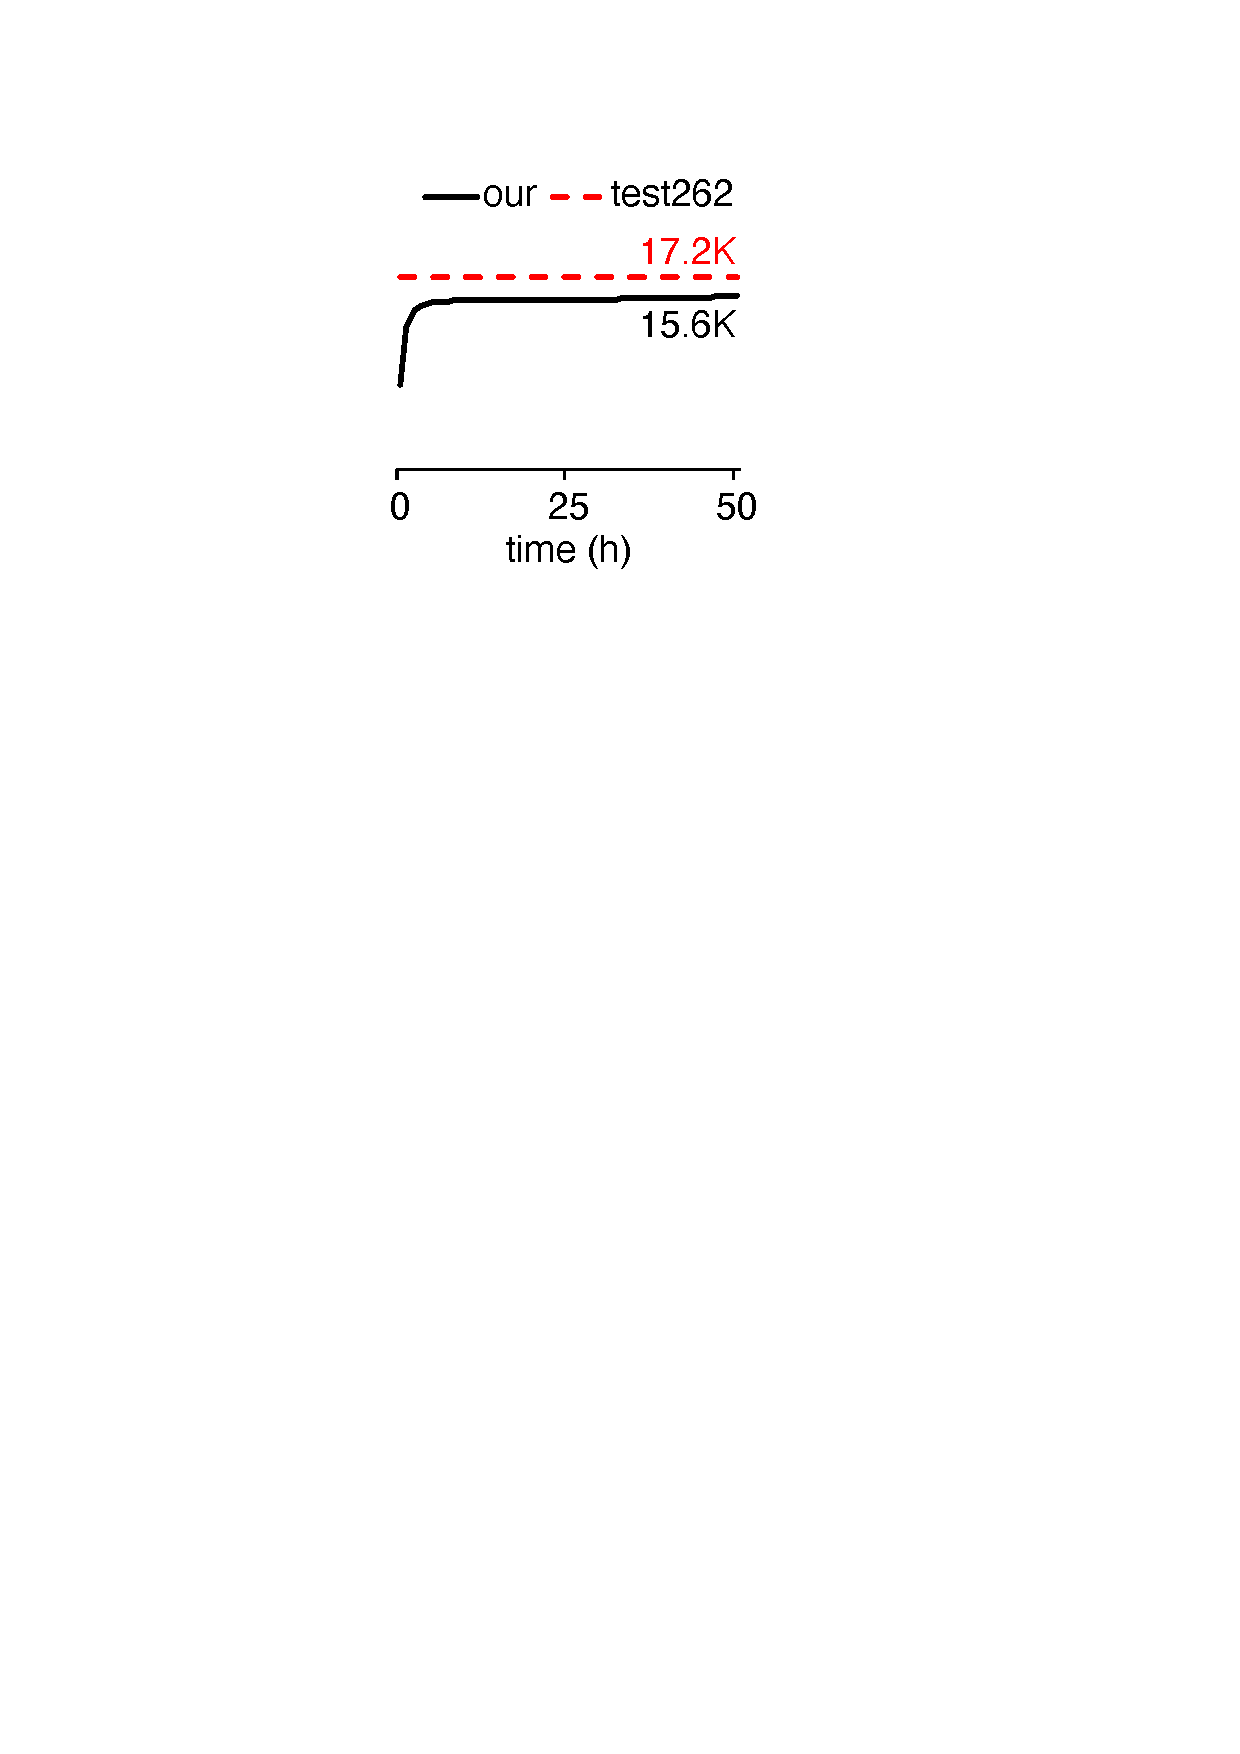
\includegraphics[width=\textwidth]{img/cov-0}
    \subcaption{Baseline.}
  \end{subfigure}
  \begin{subfigure}{0.19\textwidth}
    \centering
    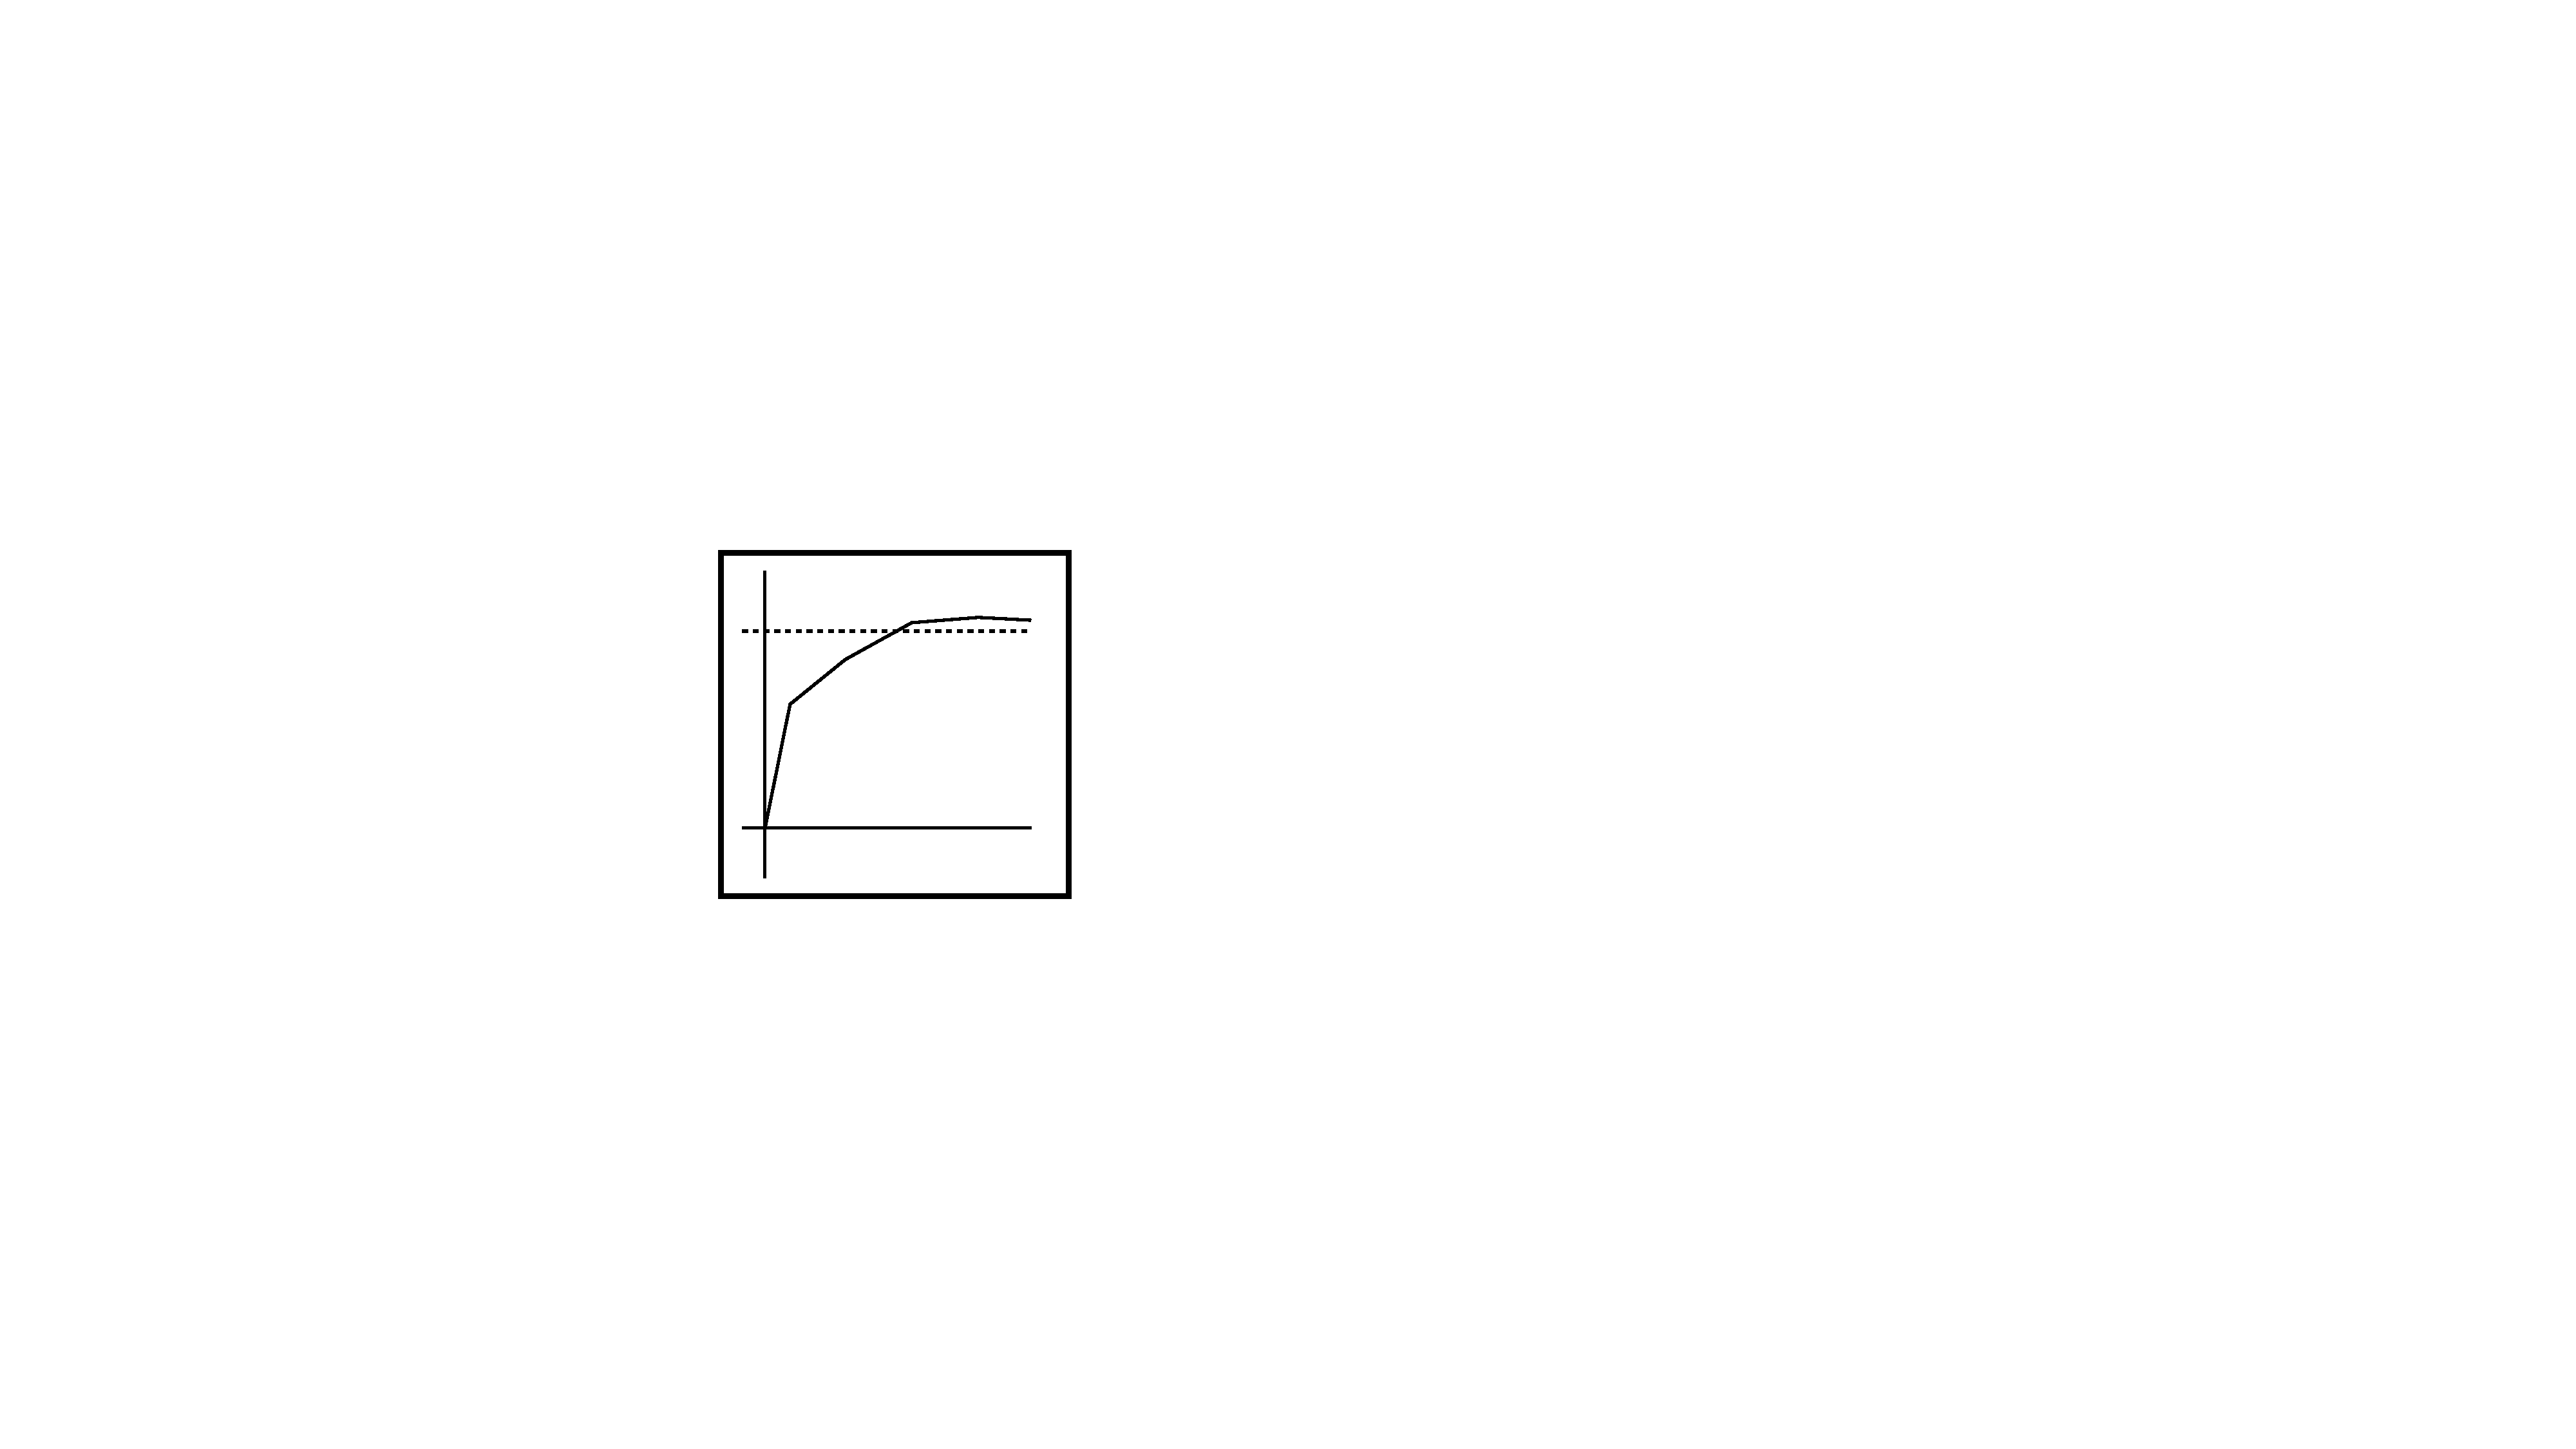
\includegraphics[width=\textwidth]{img/cov-1}
    \subcaption{1-FS}
  \end{subfigure}
  \begin{subfigure}{0.19\textwidth}
    \centering
    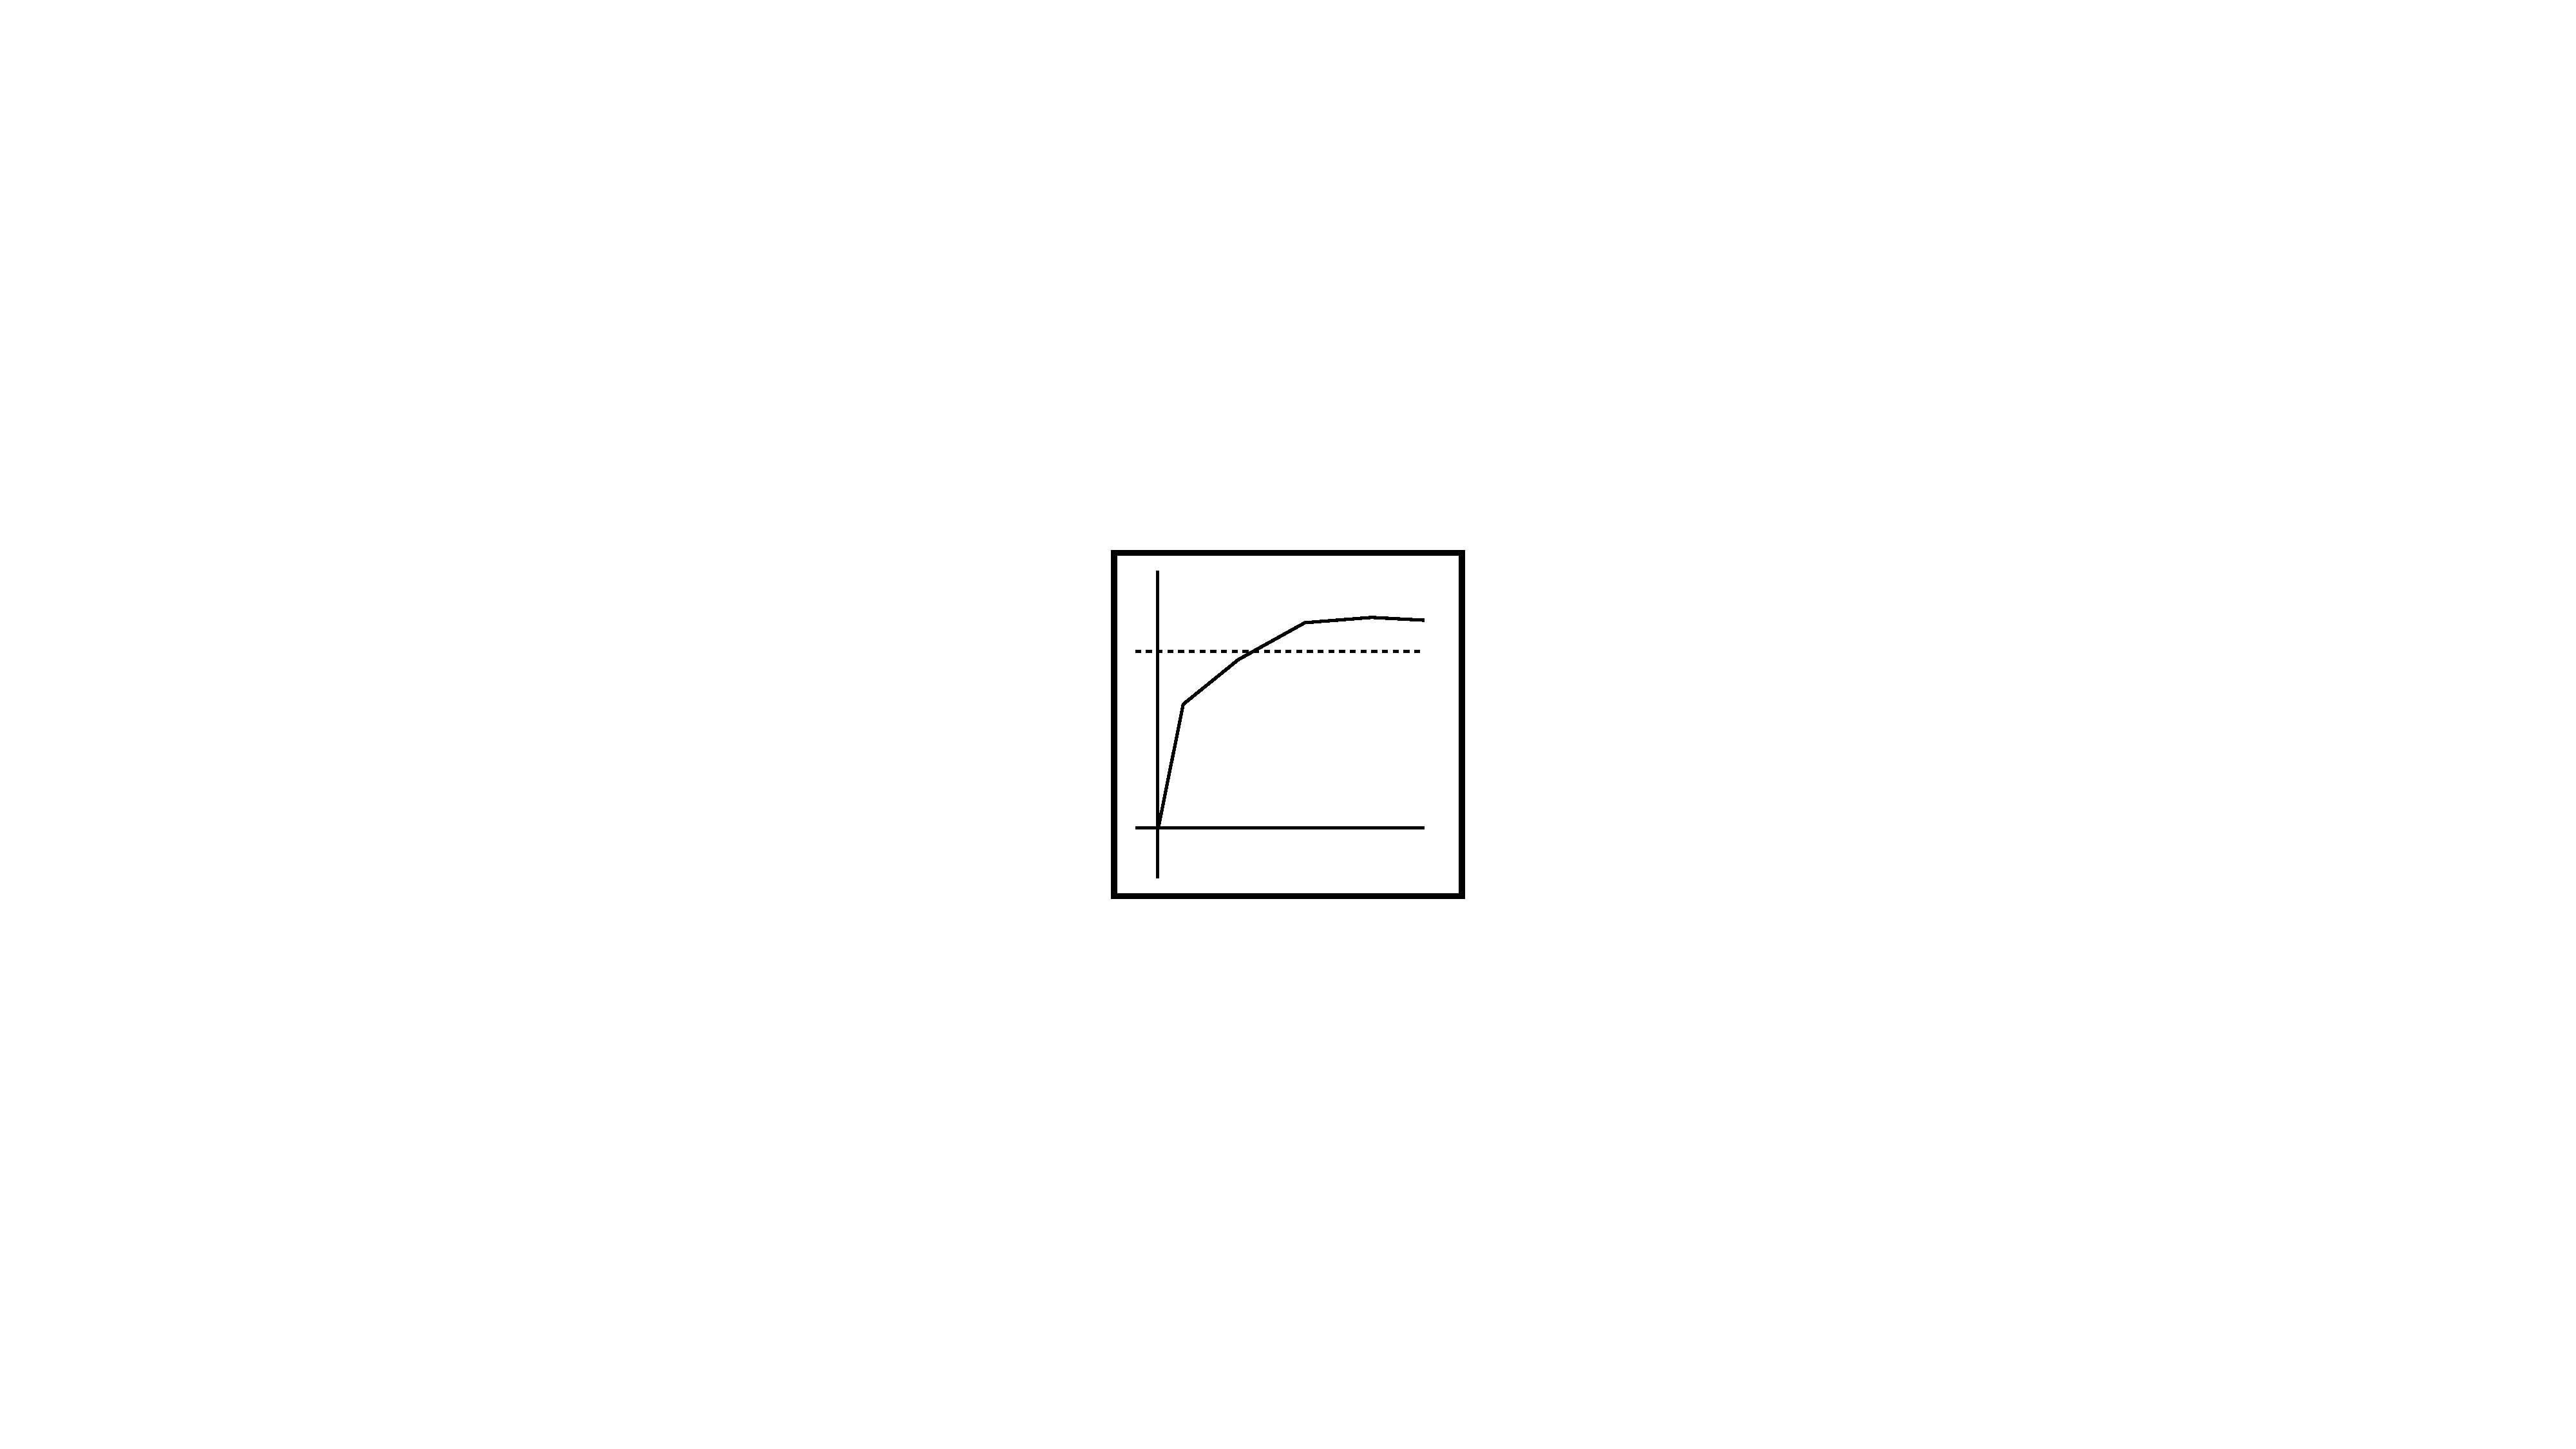
\includegraphics[width=\textwidth]{img/cov-1-fcp}
    \subcaption{1-FCPS}
  \end{subfigure}
  \begin{subfigure}{0.19\textwidth}
    \centering
    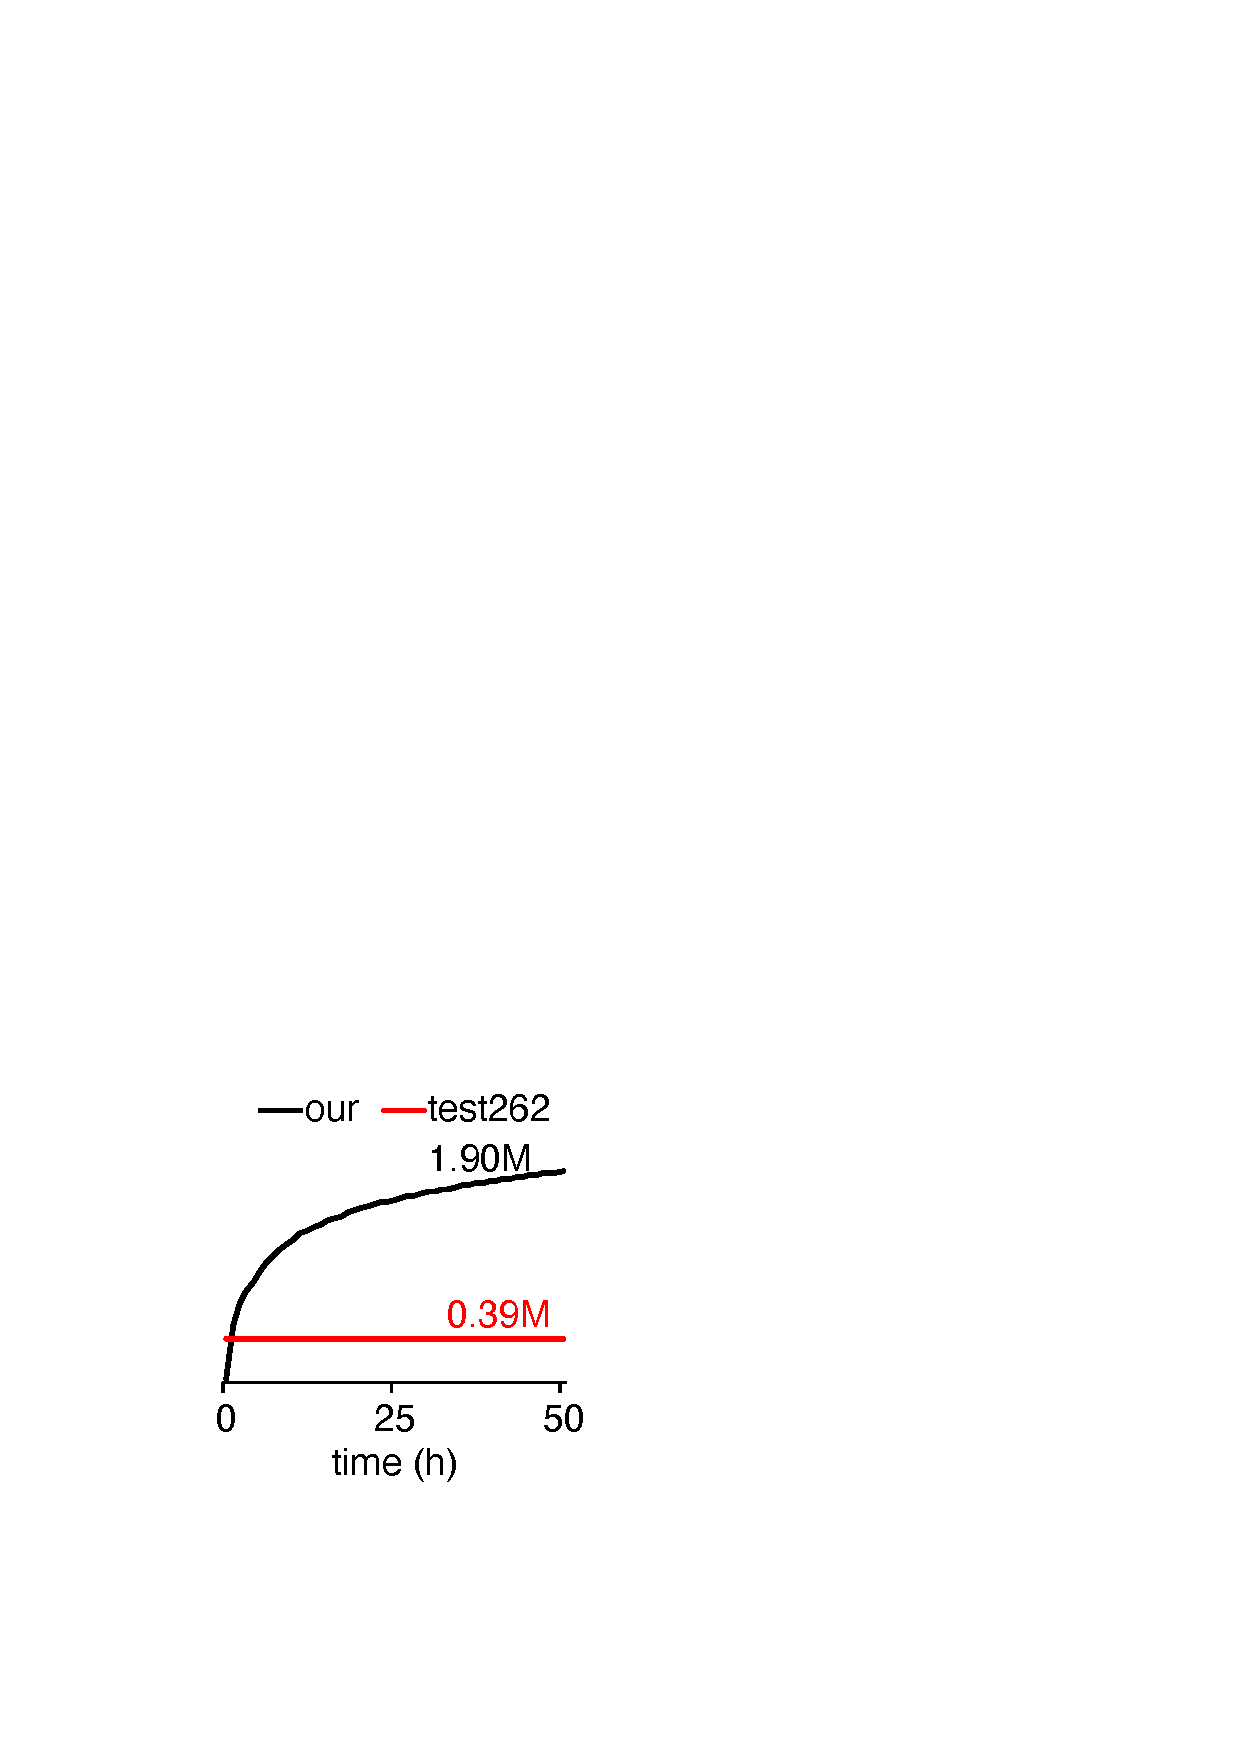
\includegraphics[width=\textwidth]{img/cov-2}
    \subcaption{2-FS}
  \end{subfigure}
  \begin{subfigure}{0.19\textwidth}
    \centering
    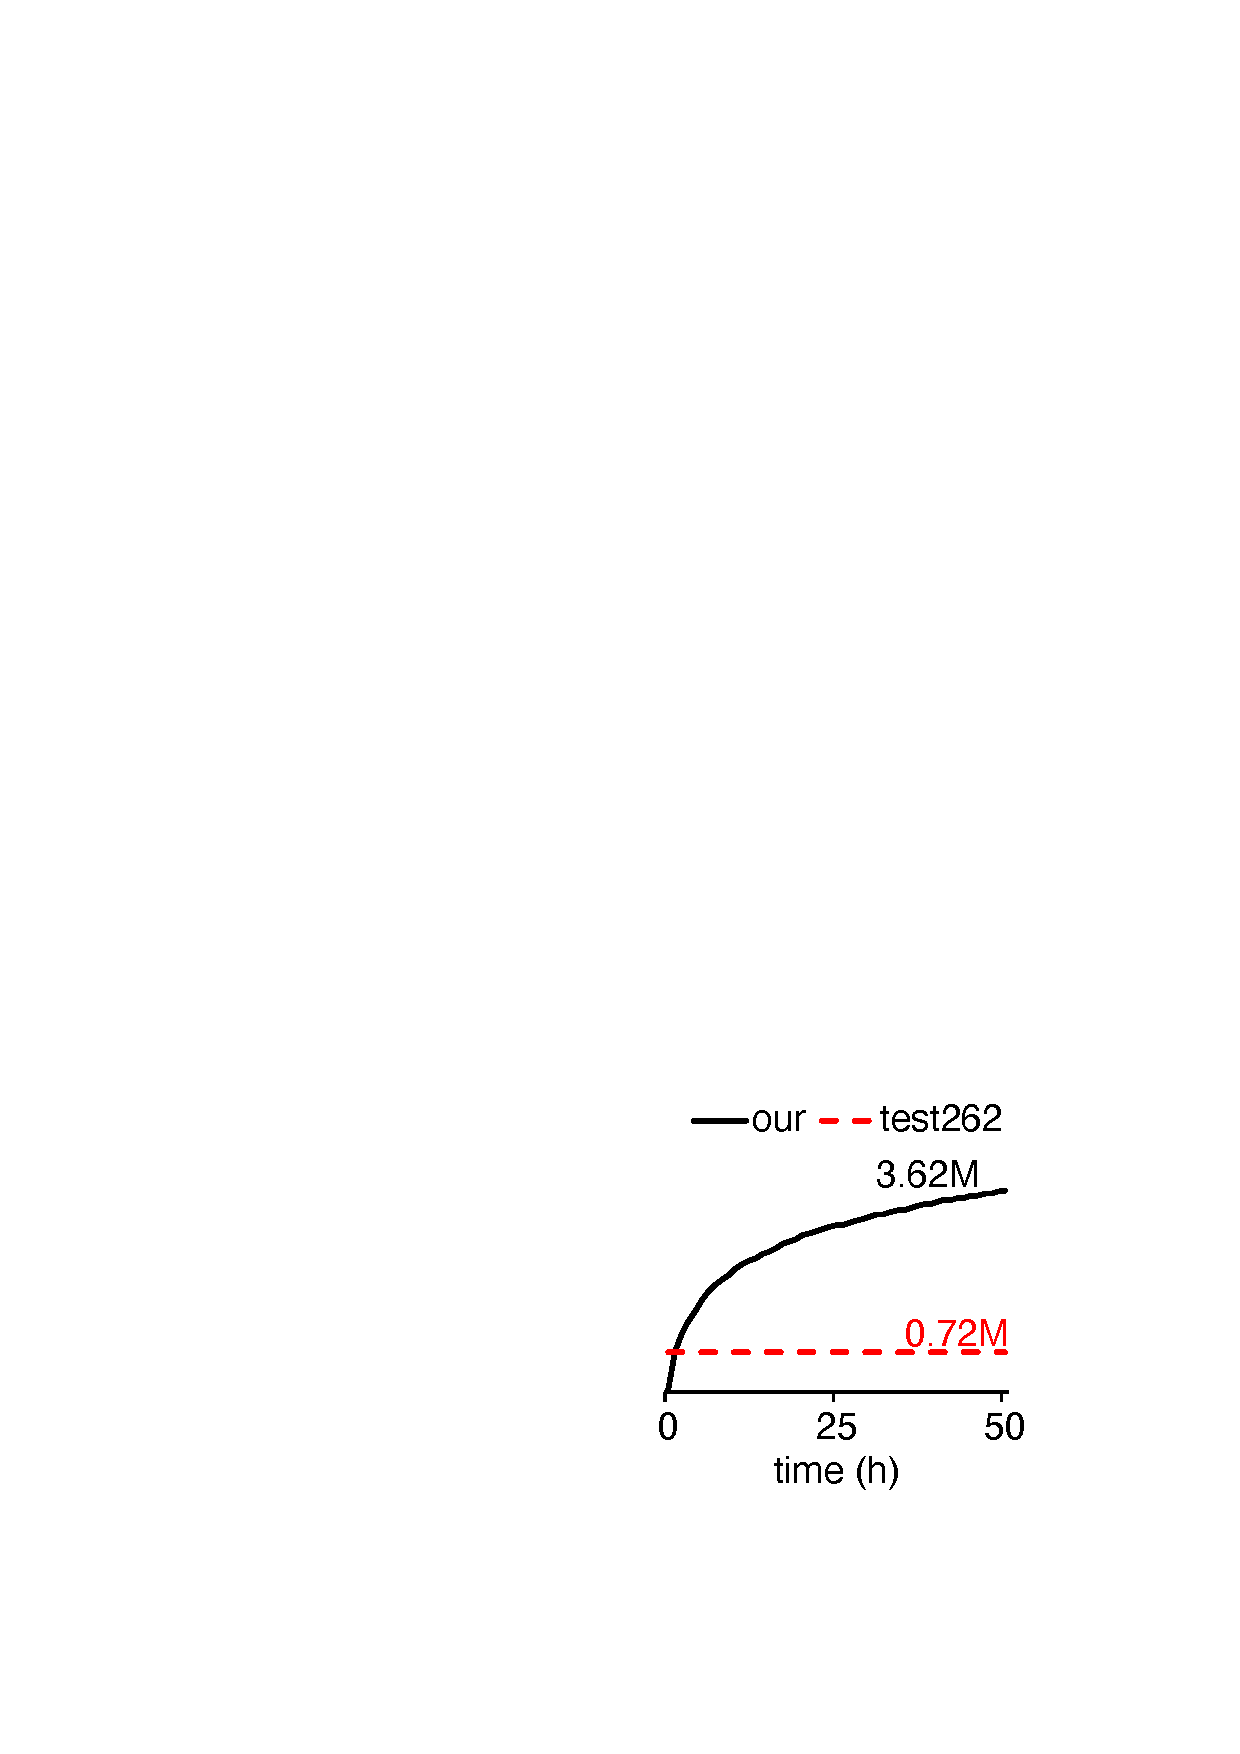
\includegraphics[width=\textwidth]{img/cov-2-fcp}
    \subcaption{2-FCPS}
  \end{subfigure}
  \caption{
    The changes of $k$-FS and $k$-FCPS node-or-branch coverages with elapse of
    time.
  }
  \label{fig:cov-time}
\end{figure}

%----------------------------------------%

\begin{figure}
  \centering
  \begin{subfigure}{0.19\textwidth}
    \venn{\x{2.7K}}{\x{14.5K}}{\x{1.0K}}
    {0.15}{0.80}{0.05}
    \subcaption{Baseline.}
  \end{subfigure}
  \begin{subfigure}{0.19\textwidth}
    \venn{\x{19.3K}}{\x{69.4K}}{\x{26.3K}}
    {0.17}{0.60}{0.23}
    \subcaption{1-FS}
  \end{subfigure}
  \begin{subfigure}{0.19\textwidth}
    \venn{\x{128.8K}}{\x{213.4K}}{\x{114.7K}}
    {0.28}{0.47}{0.25}
    \subcaption{1-FCPS}
  \end{subfigure}
  \begin{subfigure}{0.19\textwidth}
    \venn{\x{146.2K}}{\x{206.2K}}{\x{1.6M}}
    {0.07}{0.10}{0.82}
    \subcaption{2-FS}
  \end{subfigure}
  \begin{subfigure}{0.19\textwidth}
    \venn{\x{612.4K}}{\x{304.4K}}{\x{3.3M}}
    {0.15}{0.07}{0.78}
    \subcaption{2-FS}
  \end{subfigure}
  \caption{
    Venn diagrams of covered TRs of $k$-FS and $k$-FCPS node-or-branch coverages
    for Test262 and synthesized tests via $\tool$.
  }
  \label{fig:venn-test262}
\end{figure}


%----------------------------------------%

We compare the coverage of conformance tests automatically synthesized via
$\tool$ with that of Test262, the official JavaScript conformance test suite.
%
As described in Section~\ref{sec:impl}, $\tool$ is based on $\esmeta$ and only
targets the language features supported in the tool.
%
Thus, we removed \inred{23,231} out of \inred{47,141} conformance tests in
Test262 that utilize language features not supported in $\esmeta$ for a fair
comparison.
%
We measured five different $k$-FS and $k$-FCPS node-or-branch coverages for
\inred{23,910} applicable conformance tests.
%
Figure~\ref{fig:cov-time} shows the change of $k$-FS and $k$-FCPS node-or-branch
coverages with elapse of time, and the dotted line shows the coverage of Test262
in each criterion.
%
Figure~\ref{fig:venn-test262} depicts Venn diagrams of covered TRs of $k$-FS and
$k$-FCPS node-or-branch coverages for Test262 and synthesized tests via $\tool$.
%
In the baseline, the coverage of synthesized tests is less than that of Test262,
and covers only \inred{1.0K} TRs that not covered by Test262.
%
However, the coverage of synthesized exceeds the coverage of Test262 when using
feature-sensitive coverages.
%
In addition, the number of TRs only covered by synthesized tests also increases,
and the conformance tests synthesized with $2$-FCPS-TRs cover \inred{3.3M}
2-FCPS-TRs not covered by Test262.
%
We believe that this is why $\tool$ successfully detected diverse new bugs in
existing JavaScript engines and transpilers, even though most of them are
heavily tested using Test262.
